\section{Principe Générale}
Le principe de ce laboratoire est d'utiliser l'ADC que contient le PIC18F et de convertir la tension d'entrée en une valeur numérique codée sur 10 bits stockée dans une variable de 16 bits. Il sera donc important de spécifier s'il l'on désire aligner nos bits à gauche ou à droite.

\begin{figure}
\begin{center}
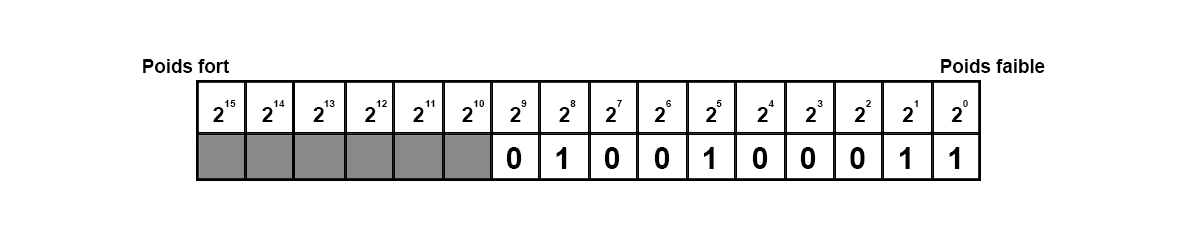
\includegraphics[scale=0.8]{images/aligndroite.png}
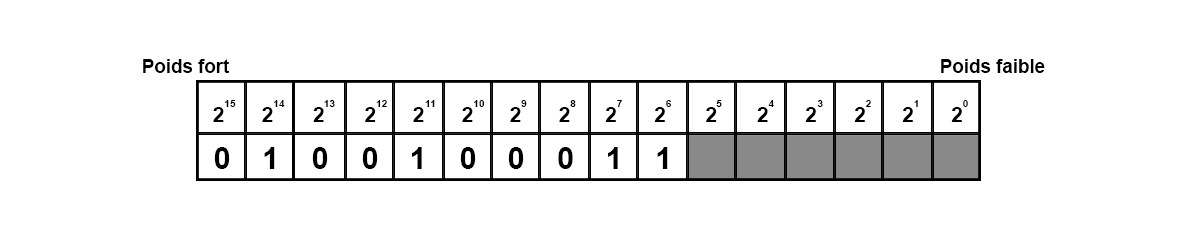
\includegraphics[scale=0.8]{images/aligngauche.png}
\end{center}
\end{figure}

\subsection{paramètres de l'ADC}

\subsubsection*{Tensions de références}
Borne de tension entre lesquelles le PIC18F convertira le signal d'entrée.(Dans ce laboratoire nous choisirons  $V_{SS}$ et $V_{DD}$ comme bornes de tensions)
\subsubsection*{Temps de conversion analogique $\rightarrow$ digitale  ($T_{AD}$)}
le $T_{AD}$  est le temps minimum nécessaire à l'ADC pour mesure un bit. Le $T_{AD}$ se configure comme un multiple en puissance de 2 de la période d'oscillation de la clock du PIC18F.
\subsubsection*{Temps d'acquisition ($T_{ACQ}$)}
le $T_{ACQ}$ est le temps minimum nécessaire pour que le condensateur CHOLD soit charger. le $T_{ACQ}$  se configure comme un multiple de 2 du $T_{AD}$. 
 